\documentclass{AuthorResponse}

%% Font Choice
%\usepackage[lining]{nunito}


%%********************************************************************************
%% Citations & Bibliography
%%****************************************
%% The choice of biblatex or natbib must match the reverenced file
%%	Biblatex requires re-including the .bib file and using \arMatchCitationNumbers
%%	natbib seems to pull everything from the aux file yay :D
%\usepackage[style=numeric, sorting=none, isbn=false, url=true,sortcites=true,maxbibnames=99]{biblatex}
%\addbibresource{Bibliography/Bibliography.bib}

\usepackage[numbers]{natbib}
\bibliographystyle{elsarticle-num}


%%********************************************************************************
%% Cross referencing from original document
%%****************************************
\arImportReferences{main}

%% Force citation numbers to match the revised document
%%	main.nocite is generated by RevisionScripts\GenerateDiff.ps1
%%	See the readme for instructions
\newcommand{\arMatchCitationNumbers}{\documentclass[preprint,3p,11pt,sort]{elsarticle}
\usepackage[utf8]{inputenc}

% Maths
\usepackage{amsmath,amssymb,amsfonts} % Equations
\usepackage{textcomp, gensymb} % Symbol: \degree

% Tables
\usepackage{multirow}

% Images
\usepackage{graphicx}
\usepackage{caption} % Improvements to figures, extends functionality with more options
\usepackage{placeins} % \FloatBarrier

% Text Modification
\usepackage[colorlinks=true, allcolors=blue]{hyperref} % Hyperlinks

% Figure & table ref
\newcommand{\figref}[1]{Fig.~\ref{#1}}
\newcommand{\tbref}[1]{Table~\ref{#1}}
\newcommand{\secref}[1]{Section~\ref{#1}}


%%%%%%%%%%%%%%%%%%%%%%%%%%%%%%%%%%%%%%%%%%%%%%%%%%%%%%%%%%%%%%%%%%%%%%%%%%%%%%%%%
%%%%%%%%%%%%%%%%%%%%%%%%%%%%%%%%%%%%%%%%%%%%%%%%%%%%%%%%%%%%%%%%%%%%%%%%%%%%%%%%%
\journal{JournalName}
\begin{document}
\begin{frontmatter}

\title{My Example Manuscript}

\nonumnote{Abbreviations: aaa}

\begin{abstract}
    This is an example manuscript. It showcases a few common latex features so that I can show how latexdiff interacts with them.
\end{abstract}

\begin{keyword}
    a \sep b \sep c \sep d
\end{keyword}

\end{frontmatter}

%%%%%%%%%%%%%%%%%%%%%%%%%%%%%%%%%%%%%%%%%%%%%%%%%%%%%%%%%%%%%%%%%%%%%%%%%%%%%%%%%
%%%%%%%%%%%%%%%%%%%%%%%%%%%%%%%%%%%%%%%%%%%%%%%%%%%%%%%%%%%%%%%%%%%%%%%%%%%%%%%%%
\section{Introduction} \label{sec:intro}
This is an example manuscript.

The structure of this article is as follows: \secref{sec:mySection} showcases the use of SSSSR sections. \secref{sec:ContentTypes} shows how to display many different types of content.


%%%%%%%%%%%%%%%%%%%%%%%%%%%%%%%%%%%%%%%%%%%%%%%%%%%%%%%%%%%%%%%%%%%%%%%%%%%%%%%%%
%%%%%%%%%%%%%%%%%%%%%%%%%%%%%%%%%%%%%%%%%%%%%%%%%%%%%%%%%%%%%%%%%%%%%%%%%%%%%%%%%
\section{Displaying Sections} \label{sec:mySection}
This section has many subsections, which I can refer to by their labels. e.g. \secref{sec:mySection}, \secref{ssec:mySubsectionA}, and \secref{ssec:mySubsectionB}. Labeling sections is optional. Labels may be anything, but must be unique (hence my naming convention).

%%%%%%%%%%%%%%%%%%%%%%%%%%%%%%%%%%%%%%%%%%%%%%%%%%%%%%%%%%%%%%%%%%%%%%%%%%%%%%%%%
\subsection{My Subsection A} \label{ssec:mySubsectionA}
Example text.


%%%%%%%%%%%%%%%%%%%%%%%%%%%%%%%%%%%%%%%%%%%%%%%%%%%%%%%%%%%%%%%%%%%%%%%%%%%%%%%%%
\subsection{My Subsection B} \label{ssec:mySubsectionB}
Example text.


%%%%%%%%%%%%%%%%%%%%%%%%%%%%%%%%%%%%%%%%%%%%%%%%%%%%%%%%%%%%%%%%%%%%%%%%%%%%%%%%%
%%%%%%%%%%%%%%%%%%%%%%%%%%%%%%%%%%%%%%%%%%%%%%%%%%%%%%%%%%%%%%%%%%%%%%%%%%%%%%%%%
\section{Displaying Different Types of Content} \label{sec:ContentTypes}


%%%%%%%%%%%%%%%%%%%%%%%%%%%%%%%%%%%%%%%%%%%%%%%%%%%%%%%%%%%%%%%%%%%%%%%%%%%%%%%%%
\subsection{Citations}
This is a citation \cite{example1}, and this is another \cite{example1,example2,example4,example5}.


%%%%%%%%%%%%%%%%%%%%%%%%%%%%%%%%%%%%%%%%%%%%%%%%%%%%%%%%%%%%%%%%%%%%%%%%%%%%%%%%%
\subsection{Lists}
An example list is as follows:

\begin{enumerate}
    \item This is a list
    \item This is a list
    \item This is a list
\end{enumerate}


%%%%%%%%%%%%%%%%%%%%%%%%%%%%%%%%%%%%%%%%%%%%%%%%%%%%%%%%%%%%%%%%%%%%%%%%%%%%%%%%%
\subsection{Figures}
This is a figure reference: \figref{fig:Example1}, and this is another \figref{fig:Example2}.

If you have mathematical symbols in your figures and you're using inkscape, you can input latex maths into the figure with: Extensions > Render > Formula (pdflatex).

\begin{figure}
	\centering
	\centerline{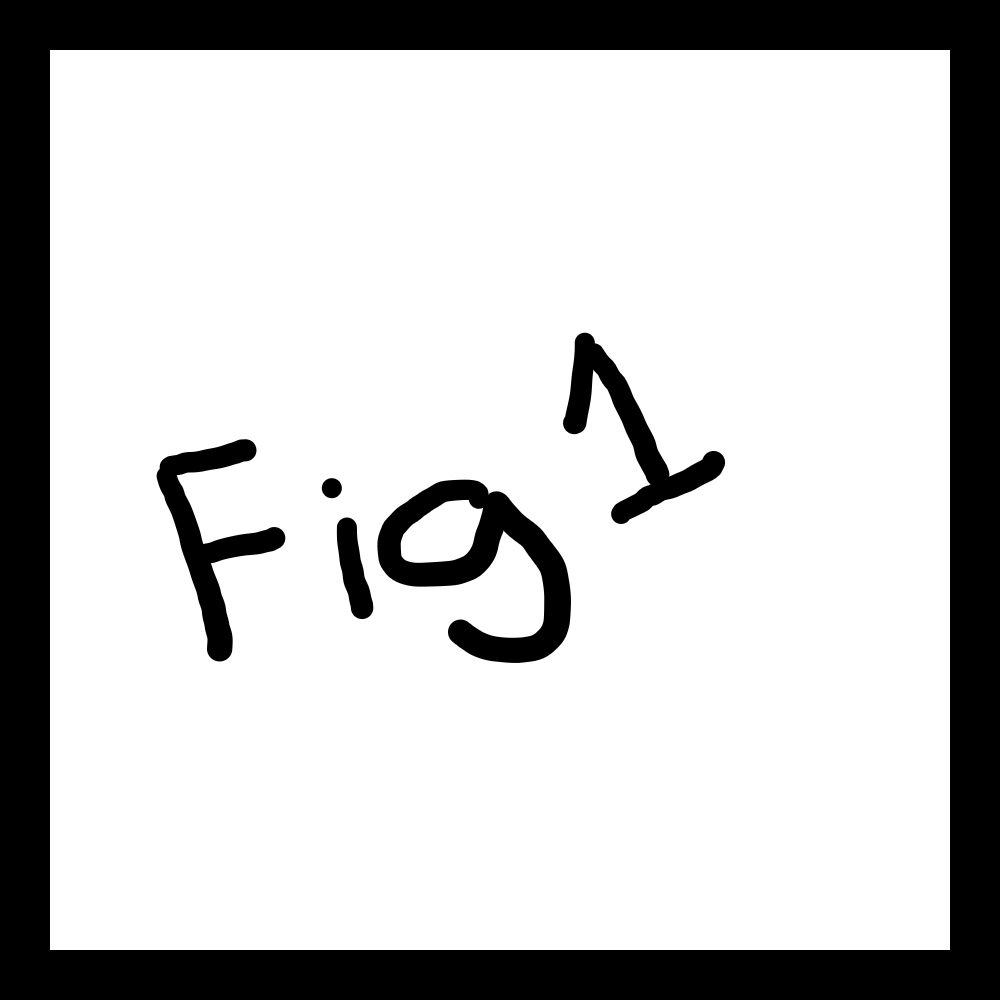
\includegraphics[width=\textwidth,keepaspectratio]{Figures/ExampleFigure1.png}}
	\caption{Embed your graphics as pdf. Lovely vector graphics! If I see any jpeg text I am sad.}
	\label{fig:Example1}
\end{figure}

\begin{figure}
	\centering
	\centerline{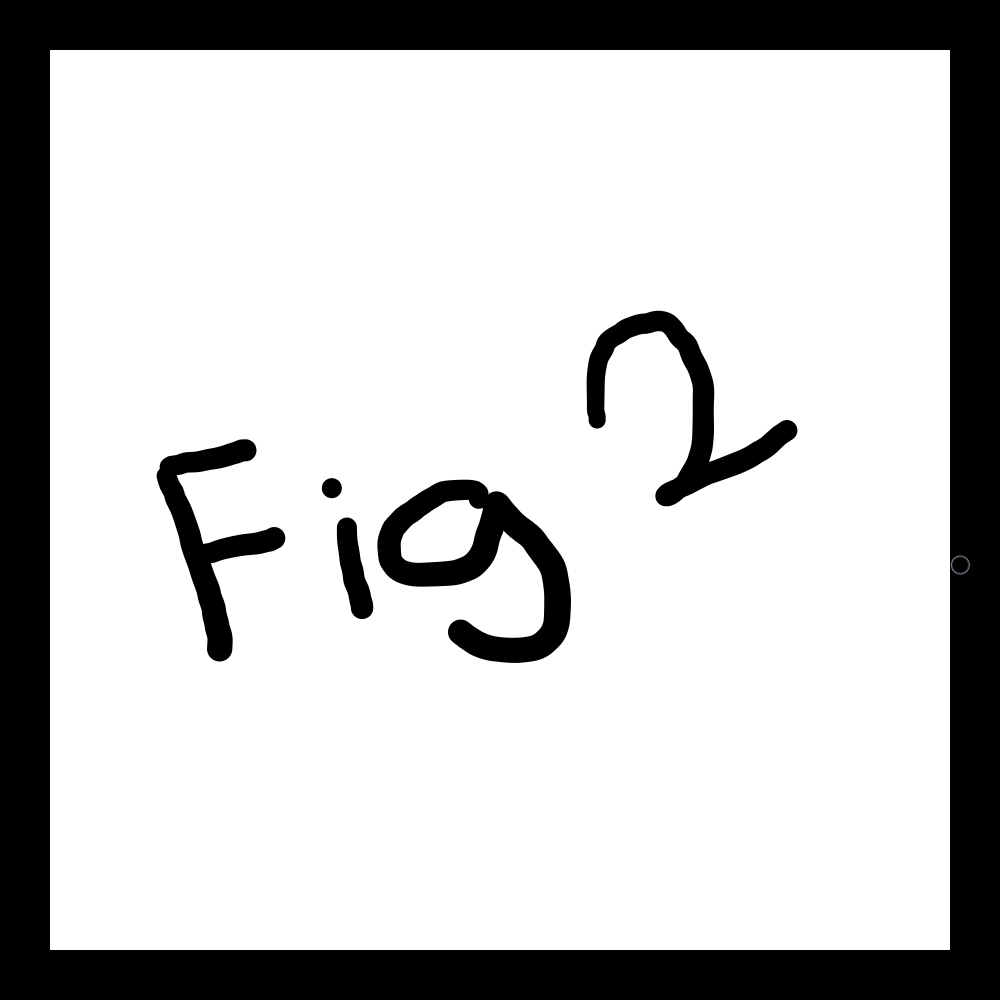
\includegraphics[width=\textwidth,keepaspectratio]{Figures/ExampleFigure2.png}}
	\caption{This is a caption.}
	\label{fig:Example2}
\end{figure}


%%%%%%%%%%%%%%%%%%%%%%%%%%%%%%%%%%%%%%%%%%%%%%%%%%%%%%%%%%%%%%%%%%%%%%%%%%%%%%%%%
\subsection{Equations}
This is an equation reference: \eqref{eq:myEq}.

\begin{equation} \label{eq:myEq}
    a = 3
\end{equation}

where $a$ is a variable.


%%%%%%%%%%%%%%%%%%%%%%%%%%%%%%%%%%%%%%%%%%%%%%%%%%%%%%%%%%%%%%%%%%%%%%%%%%%%%%%%%
\subsection{Tables}
This is a table reference: \tbref{tb:myTable}.

This is a fairly basic table. See threeparttable if you want table notes (footnotes for tables).

\begin{table}[!h]
    \centering
    \begin{tabular}{llll}
        \hline
        & & \multicolumn{2}{l}{Measurement error}\\
        Measurement & Unit & Mean & Standard deviation\\
        \hline
        $x_n$ & mm & 5.2 & 8.6\\
        $y_n$ & mm & 3.5 & 3.0\\
        $z_n$ & mm & -6.5 & 9.1\\
        $\theta_q$ & degrees & 1.6$\degree$ & 2.9$\degree$\\
        \hline
        \end{tabular}
    \caption{Average measurement error over all 99 successful measurements. $(x_n, y_n, z_n)$ are defined somewhere else. $\theta_q$ is the rotational misalignment as a quaternion angular distance.}
    \label{tb:myTable}
\end{table}


%%%%%%%%%%%%%%%%%%%%%%%%%%%%%%%%%%%%%%%%%%%%%%%%%%%%%%%%%%%%%%%%%%%%%%%%%%%%%%%%%
%%%%%%%%%%%%%%%%%%%%%%%%%%%%%%%%%%%%%%%%%%%%%%%%%%%%%%%%%%%%%%%%%%%%%%%%%%%%%%%%%
\section{Conclusions and Future Work} \label{sec:conclusions}
Thus ends the example manuscript.

I can't be bothered to recommend future work.


\FloatBarrier
%%%%%%%%%%%%%%%%%%%%%%%%%%%%%%%%%%%%%%%%%%%%%%%%%%%%%%%%%%%%%%%%%%%%%%%%%%%%%%%%%
%%%%%%%%%%%%%%%%%%%%%%%%%%%%%%%%%%%%%%%%%%%%%%%%%%%%%%%%%%%%%%%%%%%%%%%%%%%%%%%%%
\bibliographystyle{elsarticle-num}
\bibliography{Bibliography/Bibliography.bib}

%%%%%%%%%%%%%%%%%%%%%%%%%%%%%%%%%%%%%%%%%%%%%%%%%%%%%%%%%%%%%%%%%%%%%%%%%%%%%%%%%
%%%%%%%%%%%%%%%%%%%%%%%%%%%%%%%%%%%%%%%%%%%%%%%%%%%%%%%%%%%%%%%%%%%%%%%%%%%%%%%%%
\end{document}
\endinput

}


%%********************************************************************************
%% Copy user added packages and commands from main.tex
%%****************************************
\usepackage{amsmath}

%% Figure & table ref
\newcommand{\figref}[1]{Fig.~\ref{#1}}
\newcommand{\tbref}[1]{Table~\ref{#1}}
\newcommand{\secref}[1]{Section~\ref{#1}}


%%%%%%%%%%%%%%%%%%%%%%%%%%%%%%%%%%%%%%%%%%%%%%%%%%%%%%%%%%%%%%%%%%%%%%%%%%%%%%%%%
%% Start
%%%%%%%%%%%%%%%%%%%%%%%%%%%%%%%%%%%%%%%%%
\begin{document}
\pagestyle{arPageStyle}
\thispagestyle{arPageStyleFirst}
\arTitle{My Title}
\arLegend
\arMatchCitationNumbers

Dear editor and reviewers,

Thank you for your efforts in reviewing my article. I have addressed the comments to the best of my ability and updated the manuscript accordingly as detailed in this letter.

Sincerely,

Me.

%%%%%%%%%%%%%%%%%%%%%%%%%%%%%%%%%%%%%%%%%%%%%%%%%%%%%%%%%%%%%%%%%%%%%%%%%%%%%%%%%
%%%%%%%%%%%%%%%%%%%%%%%%%%%%%%%%%%%%%%%%%%%%%%%%%%%%%%%%%%%%%%%%%%%%%%%%%%%%%%%%%
\section{Reviewer \#1}
\RC This is a reviewer comment. Reviewer comments are prefixed with the command RC (reviewer comment). 

This is my response, which is formatted normally.

\RC This reviewer comment is multiple paragraphs long.

\RCC All subsequent paragraphs are prefixed with RCC (reviewer comment continued). 

My response.

\RCBlock{
	Alternatively, RCBlock can be used for reviewer comments that are multiple paragraphs long.

	RCBlock can also contain more complex typesetting.
}

\begin{RCEnv}
	The RCEnv environment is also available, if you prefer.
\end{RCEnv}

My response.


%%%%%%%%%%%%%%%%%%%%%%%%%%%%%%%%%%%%%%%%%%%%%%%%%%%%%%%%%%%%%%%%%%%%%%%%%%%%%%%%%
%%%%%%%%%%%%%%%%%%%%%%%%%%%%%%%%%%%%%%%%%%%%%%%%%%%%%%%%%%%%%%%%%%%%%%%%%%%%%%%%%
\section{Reviewer \#2}
\RC As the reviewer, I require you to change some aspect of your manuscript.

I have now changed the manuscript, as follows.

Note that the tracked changes markup can be generated automatically. See the readme for how to use the powershell script \verb|RevisionScripts/GenerateDiff.ps1| to create the tracked changes file \verb|main_diff.tex|. You can then copy paste extracts from the tracked changes file into in this file.

The optional argument of the customised quote environment is for labeling the section that the quote was extracted from. You can directly reference labels from the article, as I do here. The same ref commands can all be used: \verb|\figref|, \verb|\tbref|, \verb|\eqref|, \verb|\chapref|, \verb|\secref|, \verb|\appref|, \verb|\algoref|, \verb|\algoRefLine|, \verb|\algoRefLines|.

For any equations in the quote, the equation numbers can be made to match the article by changing the label command to \verb|\tag{\ref{}}|.

\begin{quote}[\secref{sec:ContentTypes}]
	This paragraph has mixed \DIFdel{removed} and \DIFadd{added} text.

	\DIFadd{This paragraph has been added. This is placeholder text. This is placeholder text. This is placeholder text. This is placeholder text. This is placeholder text. This is placeholder text. This is placeholder text. This is placeholder text.}

	\DIFdel{This paragraph has been removed. This is placeholder text. This is placeholder text. This is placeholder text. This is placeholder text. This is placeholder text. This is placeholder text. This is placeholder text. This is placeholder text.}

	This is an equation reference: \eqref{eq:myEq}.

	\begin{equation} \tag{\ref{eq:myEq}}
		\DIFadd{a = 2}
	\end{equation}

	\begin{equation} \tag{\ref{eq:myEq}}
		\DIFdel{a = 3}
	\end{equation}
	
	where $a$ is a variable.
\end{quote}

Alternatively, format the quote like this

\begin{quote}[Equation \ref{eq:myEq}]
	\begin{equation} \notag
		\DIFadd{a = 2}
	\end{equation}

	\begin{equation} \notag
		\DIFdel{a = 3}
	\end{equation}
\end{quote}

\RC Change some parts of the abstract.

I have now updated the abstract. Because the abstract does not have a label, we can just type `Abstract' as the quote origin.

\begin{quote}[Abstract]
	This paragraph from the \DIFdel{summary} \DIFadd{abstract} has been \DIFdel{modified} \DIFadd{changed}.
\end{quote}


\RC Change the wording in the figure captions because I prefer this other word.

I have now updated the figure caption.

\begin{quote}[\figref{fig:Example1} Caption]
	The figure caption has been \DIFdel{modified} \DIFadd{changed}.
\end{quote}


\RC Figure x is difficult to interpret. Make it more clear.

I have now updated the figure. To quote figures, copy only the \verb|\includegraphics| command, not the entire float environment. I also copy the caption below it.

\begin{quote}[\figref{fig:Example2}]
	\centerline{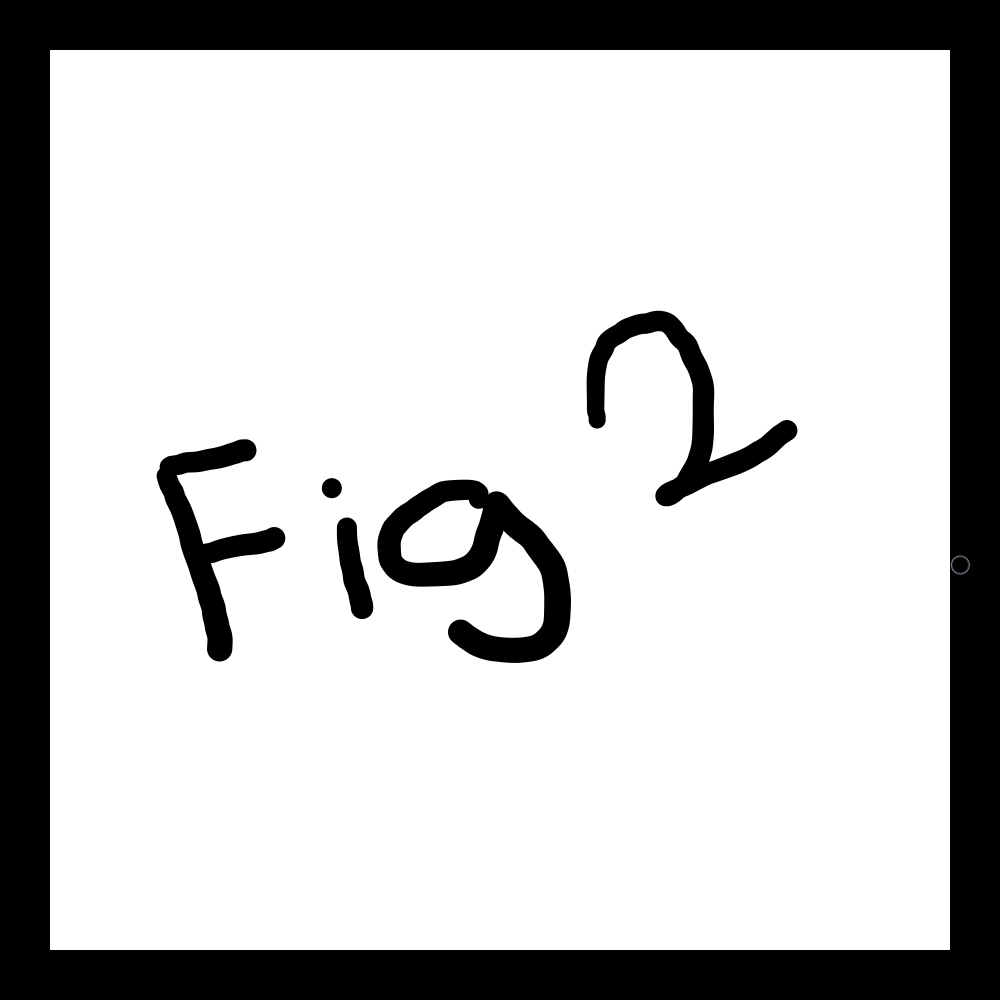
\includegraphics[width=0.5\columnwidth,keepaspectratio]{Figures/ExampleFigure2.png}}
	Figure \ref{fig:Example2}: This is a very long caption that takes up multiple lines.
\end{quote}

Doing all of this is a bit of work, but keep in mind that the goal is to make it very clear exactly how you have addressed each of the reviewers comments, that you can get your work accepted without any back-and-forth. Use this template to achieve that goal.


%%%%%%%%%%%%%%%%%%%%%%%%%%%%%%%%%%%%%%%%%%%%%%%%%%%%%%%%%%%%%%%%%%%%%%%%%%%%%%%%%
%%%%%%%%%%%%%%%%%%%%%%%%%%%%%%%%%%%%%%%%%%%%%%%%%%%%%%%%%%%%%%%%%%%%%%%%%%%%%%%%%
\end{document}

